\documentclass{article}
\usepackage[serbian]{babel}
\usepackage[utf8]{inputenc}
\usepackage{fancyhdr}
\usepackage{lipsum}
\usepackage{graphicx}
\graphicspath{ {./images/} }
\usepackage{ulem}
\usepackage{wrapfig}
\usepackage{amsmath}
\usepackage{amssymb}
\usepackage{subcaption}
\usepackage{hyperref}

\title{BROJ $e$ I PRIMENA U FINANSIJAMA\\\large{Seminarski rad u okviru kursa}\\\large{Tehničko i naučno pisanje}\\ \large{Matematički fakultet}}

\author{}
\begin{document}

\maketitle

\begin{center}
    

\section*{\large{ANASTASIJA DIVJAK}}

\paragraph{\normalfont{mi22206@alas.matf.bg.ac.rs}}

\section*{\large{NIKOLINA MILENKOVIĆ}}

\paragraph{\normalfont mi22142@alas.matf.bg.ac.rs}

\section*{\large{KRISTINA MILENKOVIĆ}}

\paragraph{\normalfont mi22117@alas.matf.bg.ac.rs}

\section*{\large{NIKOLA JOVANOVIĆ}}


\paragraph{\normalfont {mi22122@alas.matf.bg.ac.rs}}



\paragraph{\\}
\end{center}
\paragraph{\textbf{REZIME: }\normalfont { Kada je otkriven 1618. godine, broju $e$ nije pridavan veliki značaj. Njegovu pravu ulogu otkriva znatno kasnije švajcarski matematičar Leonard Ojler. Ova konstanta iznosi $e$  2,71828... i predstavlja osnovu prirodnog logaritma. Veliku primenu ima i van matematike, a jedna od njegovih najbitnijih primena je u finansijama. Smatra se da je kao prvobitni problem broja $e$ upravo bio problem vezan za finansije. }}
\paragraph{\normalfont{\textbf{KLJUČNE REČI}: broj $e$, prirodan logaritam, finansije, Leonard Ojler}}




\newpage{}

\title{\Large\centering{{SADRŽAJ}}}

\section{\LARGE Rezultati istraživanja i diskusija}
    \subsection{\Large\normalfont Istorija broja $e$ \hspace{8.1cm} 3}
    \subsection{\Large\normalfont O Leonardu Ojleru \hspace{7.2cm} 3}
    \subsection{\Large\normalfont Osobina broja $e$ \hspace{7.88cm} 4}
    \subsection{\Large\normalfont Ojlerov identitet \hspace{7.7cm} 6}
    \subsection{\Large\normalfont Ojlerova kružnica \hspace{7.5cm} 7}
    \subsection{\Large\normalfont Primena broja $e$ u finansijama \hspace{4.85cm} 8}
    \subsection{\Large\normalfont O Bernuliju \hspace{8.7cm} 8}
    \subsection{\Large\normalfont Značaj u finansijama \hspace{6.75cm} 8}
    \subsection{\Large\normalfont Reference \hspace{9.1cm} 9} 



\newpage{}
\pagestyle{fancy}
\fancyhead{}
\fancyhead[RO,LE]{\textbf{Broj $e$ i primene u finansijama}}

\title{\Large\centering{{REZULTAT ISTRAŽIVANJA I DISKUSIJA}}}

\section*{\uline{Istorija broja $e$}}
\paragraph{\normalfont{Broj e se prvi put pojavljuje 1618.godine u logaritamskim tablicama tj. nakon Neperovog otkrića integrala. Tada mu nije pridavan veliki znacaj i njegovu ulogu u matematici i drugim oblastima otkriva znatno kasnije švajcarski matematičar i fizičar Leonard Ojler.\cite{elementarium}}}

\paragraph{\normalfont{Naime, u 17.veku švajcarski matematičar Danijel Bernuli ispitivao je kamatnu stopu i različite dohotke na osnovu učestalosti ulaganja. Ono što je zaključio, a što se sad smatra originalnim problemom broja $e$, jeste da se dobija bolji rezultat ako se češće ulaže novac 
i uzima kamata.}}

\paragraph{\normalfont{Pedesetak godina nakon ovoga, Ojler je napokon izračunao vrednost broja $e$ s obzirom da je Bernuli znao samo da se taj broj nalazi izmedju 2 i 3. Osim što ga je izračunao on je pronašao i formulu kojom je dokazao da je ovaj broj iracionalan.\cite{iserbia}\\}}


\begin{wrapfigure}{r}{0.5\textwidth}
  \begin{center}
    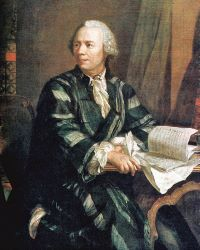
\includegraphics[width=0.48\textwidth]{lojlermodified.jpg}
  \end{center}
  \caption{Leonardo Ojler}
\end{wrapfigure}

\section*{\uline{O Leonardu Ojleru}}

Leonard Ojler rođen je u Bazelu 15. aprila 1707. godine.
Bio je jedan od najznačajnijih matematičara 18. veka.
Najviše je doprineo u matematičkoj notaciji jer je prvi počeo
da koristi $f(x)$ za zapis funkcije, moderan zapis trigonometrijskih funkcija, $e$, $\Sigma$
za sumu, $i$ kao imaginarnu jedinicu.
Pokazao je da se najkraće rastojanje izmedju dve tačke na zakrivljenoj površi pretvara u duž ukoliko se ta površ projektuje na ravan.
Među manje poznatim Ojlerovim doprinosima nalazi se pokušaj formulisanja teorije muzike u potpunosti zasnovan na matematičkim idejama, koji je napravio napisavši 1739. godine "Tentamen novae theoriae musicae",a zatim i brojna druga dela.
\newpage{}
	
	
	\section*{\underline{Osobine broja e}}
	
	
	Broj e, koji još nazivamo i Ojlerov broj ili Neperova konstanta, je konstanta koja predstavlja osnovu prirodnog logaritma. Ovaj broj osim što je iracionalan i realan takodje je i transcedentan i njegova približna vrednost iznosi
	
	
	\begingroup
	\centering
	\[ e\approx 2,71828...\]
	\endgroup
	\vspace{5mm}
	
	\begin{wrapfigure}{l}{0.25\textwidth}
		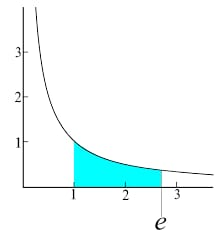
\includegraphics[scale = 0.5]{1.png}
		\caption{Broj e}
		\label{fig:br}
	\end{wrapfigure}
	On predstavlja prirodan rast tako da svoju primenu nalazi u bilo kakvom eksponencijalnom rastu bilo da je u pitanju populacija, novac ili nešto drugo. Ojler je broj e (\ref{fig:br}) izračunao kao vrednost kojoj se približava broj
	\newline
	
	\begingroup
	\centering
	
	$( 1 + \frac{1}{n} )^n$
	
	\endgroup 
	\vspace{5mm}
	
	kada se broj n povećava. Ovo će biti objašnjeno tabelama \ref{tab:tabela}. 
	\vspace{3cm}
	
	\begin{center}

           
		\begin{tabular}{|c|c|c|c|c|c|c|c|c|c|}
			\hline 
			n & 0 & 1 & 2 & 3 & 4 & 5 & 6 & 100 & 1000 \\
			\hline
			$( 1 + \frac{1}{n} )^n$ &   &   &   &   &   &   &   &   &   \\
			\hline

		\end{tabular}
          \label{tab:tabela}
	\end{center}
	
	
	\begin{center}
		\begin{tabular}{|c|c|c|c|c|c|c|c|c|c|}
			\hline 
			n & 0 & 1 & 2 & 3 & 4 & 5 & 6 & 100 & 1000 \\
			\hline
			$( 1 + \frac{1}{n} )^n$ & - & 2 & 2,25 & 2,3704 & 2,4414 & 2,4883 & 2,5216 & 2,7048 & 2,7169 \\
			\hline
   
		\end{tabular}
	\end{center}
\vspace{5mm}

\begin{align}
    
Što je veći broj n to smo bliži broju e (\ref{fig:vrednost}). Pošto je ovo beskonačan niz, broj e se može predstaviti kao granična vrednost (\ref{fig:niz}) tog niza 

 \end{align}
\begin{center}
	
	$\lim_{n\to\infty} ( \, 1 + \frac{1}{3n} 	) \,^n$

 \end{center}
\vspace{10mm}	\cite{krug}
	
	Uradićemo primer  $\lim_{n\to\infty} ( \, 1 + \frac{1}{3n} 	) \,^n$
\vspace{10mm}	
	\begin{center}
	    
	
	$\lim_{n\to\infty} ( \, 1 + \frac{1}{n} 	) \,^n =\lim_{n\to\infty} ( \, 1 + \frac{1}{3n} ) \,^\frac{3n}{3}= (\lim_{n\to\infty} ( \, 1 + \frac{1}{3n} ) \,^3n)^\frac{1}{3}= e^\frac{1}{3}$

\end{center}	
	

	
	\begin{figure}[h]
		
		\begin{subfigure}{0.5\textwidth}
			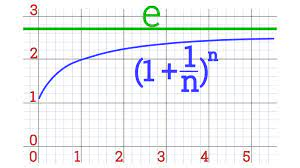
\includegraphics[width=0.9\linewidth, height=4cm]{image.png} 
			\caption{Granična vrendost datog niza}
			\label{fig:vrednost}
		\end{subfigure}
		\begin{subfigure}{0.5\textwidth}
			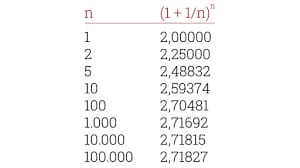
\includegraphics[width=0.9\linewidth, height=4cm]{2.png}
			\caption{Vrednosti datog niza}
			\label{fig:niz}
		\end{subfigure}
		\label{fig:image2}
	\end{figure}
	\vspace{10mm}
	
	Takodje, ovaj broj je moguće predstaviti i kao sumu beskonačnog niza

 \vspace{10mm}
	\[ e= \sum_{n=0}^{\infty} \frac{1}{n!} = \frac{1}{0!} + \frac{1}{1!} + \frac{1}{2!} + \frac{1}{3!} + ... \]
	\vspace{5mm}
	
	Zbir prvih šest članova ovog niza iznosiće
	
	\[ 1 + 1 + \frac{1}{2} + \frac{1}{6} + \frac{1}{24} + \frac{1}{120} = 2,718055556 \]
	\vspace{5mm}\cite{zavod}
	
	U nastavku biće predstavljen jedan zanimljiv primer vezan za broj e. Uzećemo broj 10 za početak. Podelićemo ga na dva jednaka dela tj.
	
	\[ 10 : 2 = 5 \]
	\vspace{5mm}
	
	Nakon ovoga, ta dva dela ćemo pomnožiti
	
	\[ 5 * 5 = 25 \]
	\vspace{5mm}
	
	Sad ćemo ponoviti postupak s tim što ćemo broj 10, umesto na dva, podeliti na 3 dela
	
	\[ 10 : 3 = 3\frac{1}{3} \]
	\vspace{5mm}
	
	Množimo delove koje smo dobili
	
	\[  3\frac{1}{3} *  3\frac{1}{3} *  3\frac{1}{3} = 37,03... \]
	\vspace{5mm}
	
	Isto radimo za četiri dela
	
	\[ 10 : 4 = 2,5 \]
	
	\[ 2,5^4 = 39,0625\]
	\vspace{5mm}\cite{matematika} 
	
	Šta je poenta ovog računanja? Da bi proizvod jednakih delova nekog broja bio maksimalan, ti delovi moraju biti što bliži broju e.
	\section*{\uline{Ojlerov indetitet}}
\paragraph{\normalfont{Osim što se može prestaviti gore navedenim izrazima, broj $e$ srećemo i u Ojlerovom indetitetu. To je ustvari naziv za formulu: $$e^{i\phi}=\cos\phi+\sin\phi$$
koja predstavlja vezu između trigonometrijskih funkcija i kompleksnih brojeva. Iako je prvobitna pretpostavka bila $\in \mathbb{R}$, jednačina važi i za $\phi\in\mathbb{C}$.}}
\paragraph{\normalfont{Za ugao $\phi=\pi$ dobija se indetitet $e^{i\pi}=-1$ (slika\ref{fig:kruznica sa vrednostima}) ili malo drugačiji oblik $e^{i\pi}+1=0$
\cite{alas}}}
\paragraph{\normalfont{Ovo se često naziva najdivnijom formulom matematike jer povezuje fundamentalne brojeve $i, \pi, e, 1$, i $0$, osnovne matematičke radnje, sabiranje, množenje i stepenovanje, i najvažniju relaciju $=$ i ništa više.
}}
\begin{figure}[h]
    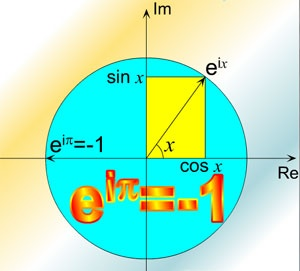
\includegraphics[width=4.98cm, height=4.5cm]{ojlerova_kruznica1.jpg}
    \centering
    \caption {Vrednosti broja $e$ na trigonometrijskoj kržnici}\label{fig:kruznica sa vrednostima}
\end{figure}
\section*{\uline{Ojlerova kružnica}}
\paragraph{\normalfont{Ojlerova kružnica, još nazivana kružnica devet tačaka, zanimljiva je u geometriji, a predstavlja kružnicu koja se može konstruisati za svaki trougao.}}Ime je dobila po tačkama koje sadrži:
\begin{itemize}
\item[-] Podnožja visina trougla, iliti tri tačke u kojima se normale iz temena trougla seku sa stranicama na koje su normalne.
\item[-] Podnožja težišnih duži trougla. Težišna duž je duž koja spaja teme trougla i središte nasprame strane. Ovih tačaka ima takođe tri.
\item[-] Sredine rastojanja ortocentra trougla od svakog temena.
\end{itemize}
 Primer na kome se vidi svih devet tačaka je slika\ref{fig:kruznica}. Gde su tačke D, E i F sredine stranica trougla. Tačke G, H i I su podnožja visina. Tačke J, K i L su sredine duži koje spajaju ortocentar S (presek visina) sa svakim temenom. 
\begin{figure}[h]
    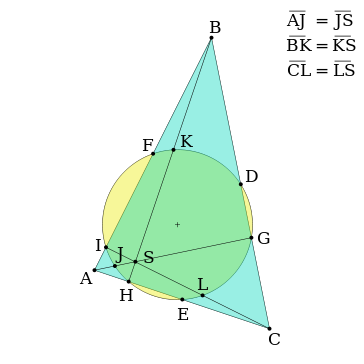
\includegraphics[width=8cm]{ojlerova_kruznica2.png}
  \caption {Ojlerova kružnica konstruisana nad trouglom}\label{fig:kruznica}
\end{figure}  
\pagestyle{fancy}
\fancyhead{}
\fancyhead[RO,LE]{\textbf{Broj $e$ i primene u finansijama}}
\section*{\uline{Primena broja e u finansijama}}
\begin{wrapfigure}{r}{0.5\textwidth}
  \begin{center}
    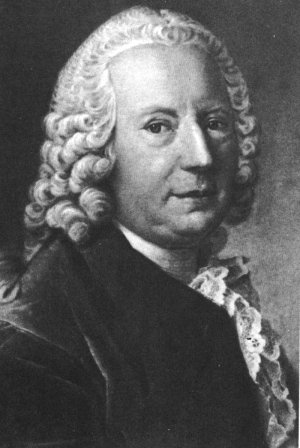
\includegraphics[width=0.33\textwidth]{bernuli.jpg}
  \end{center}
  \caption{Danijel Bernuli}
\end{wrapfigure}
\paragraph{\normalfont{Vrednost broja $e$ u početku je računata u bankarske svrhe.
Kao što je rečeno, smatra se da je problem broja $e$ bio vezan za finansije. Danijel Bernuli ispitivao je kamatnu stopu i različite dohotke na osnovu učestalosti ulaganja.}}
\section*{\uline{O Bernuliju}}
Sticao je znanja iz matematike i prirodnih nauka, predavao je matematiku, anatomiju, botaniku i fiziku. Bio je prijatelj Leonarda Ojlera, zajedno su sarađivali na više polja matematike i fizike. Različiti problemi koje je pokušavao da razreši (teorija elastičnosti, mehanika talasa) nagnali su ga da razvije takav matematički aparat kao što su diferencijlne jednačine i redovi.
\section*{\uline{Značaj u finansijama}}
Pretpostavimo da u banku ulažemo sumu novca h. Ako bi banka davala 100\%-tnu kamatu,
za godinu dana mogli bismo da podignemo sumu novca 2h. Ukoliko bismo posle pola
godine podigli novac i opet ga uložili nakon godinu dana suma novca iznosila bi
\begin{equation} (1+\frac{1}{2})^2*x. \end{equation}
Ako bismo ovaj postupak primenjivali svaki dan, nakon godinu dana suma novca
iznosila bi $((1+\frac{1}{365})^{365}*x)$. Sad, postavlja se pitanje koliko novca bi mogli da zaradimo kada bi banka računala složen interes $n$ beskrajno malim vremenskim intervalima tzv. „neprekidno kapitalisanje“? Odgovor je:
\begin{equation} \lim_{n \rightarrow \infty} (1+\frac{1}{n})^n=e \end{equation}
Dakle, značaj se ogleda u tome što smo na osnovu poznavanja broja $e$ zaključili da zarada ne zavisi samo od količine novca koji ulažemo, već i od učestalosti ulaganja (odnosno sa češćim ulaganjem veća je i zarada).\cite{alas}
\section*{\uline {Zaključak}}
\paragraph{\normalfont{U cilju približavanja teme čitaocu i lakšeg razumevanja, ovaj rad izrađen je kroz teorijska objašnjenja i praktične primere. Fokus ovog rada bio je na jednoj konstanti čija se važnost i primena ne ogledaju samo na polju matematike već i u svakodnevnom životu. Iako mi toga možda nismo svesni, ovo otkriće u matematici doprinelo je razvoju mnogih drugih sfera kao što su biologija, fizika, hemija, bankarstvo, računovodstvo...Broj $e$ u ekonomiji zapravo predstavlja prvu oblast obračuna složenih kamata, dok u statistici igra bitnu ulogu u teoriji verovatnoće i eksponencijalne funkcije. Pošto se broj $e$ kao zasebna tema ne izučava toliko u školi već se spominje kroz druge pojave, autori se nadaju da su kroz ovaj су kroz rad uspeli da objasne značaj i istorijski razvitak ovog broja.}}

\begin{thebibliography}{7}
\bibitem{zavod} Vene T. Bogosavov, Zbirka rešenih zadataka iz matematike 3, za 3. razred srednje škole, Zavod za udzbenike i nastavna sredstva, Beograd, 2013.\\
\bibitem{krug} S. Ognjanović, Ž. Ivanović, Krugova zbirka zadataka i testova iz matematike za 3. razred gimnazija i tehničkih škola, Krug, Beograd, 2010.\\
\bibitem{elementarium}\url{ http://elementarium.cpn.rs/teme/sedam-najlepsih-brojeva/} \\
\bibitem{matematika}\url{https://www.matematika.edu.rs/saznajte-zanimljivosti-o-broju-e/}\\
\bibitem{iserbia}\url{https://www.iserbia.rs/da-li-ste-znali/dan-broja-pi-broj-e-314-271/}\\
\bibitem{poincare}\url{http://poincare.matf.bg.ac.rs/}\\
\bibitem{alas}\url{http://alas.matf.bg.ac.rs/~mn06070/Broj_e.pdf/}
\end{thebibliography}.
\end{document}
